In this section we will solve $\TSP$ instances. 
For the project, we used Gurobi with its Python-API in a Jupyter Notebook, see \autoref{sec:code_project}
\subsection{First instance}
First, have a look at our \enquote{good} graph $(V,E_G)$:
\vspace{5pt}\\\scalebox{0.6}{
\begin{minipage}{\textwidth}
\centering
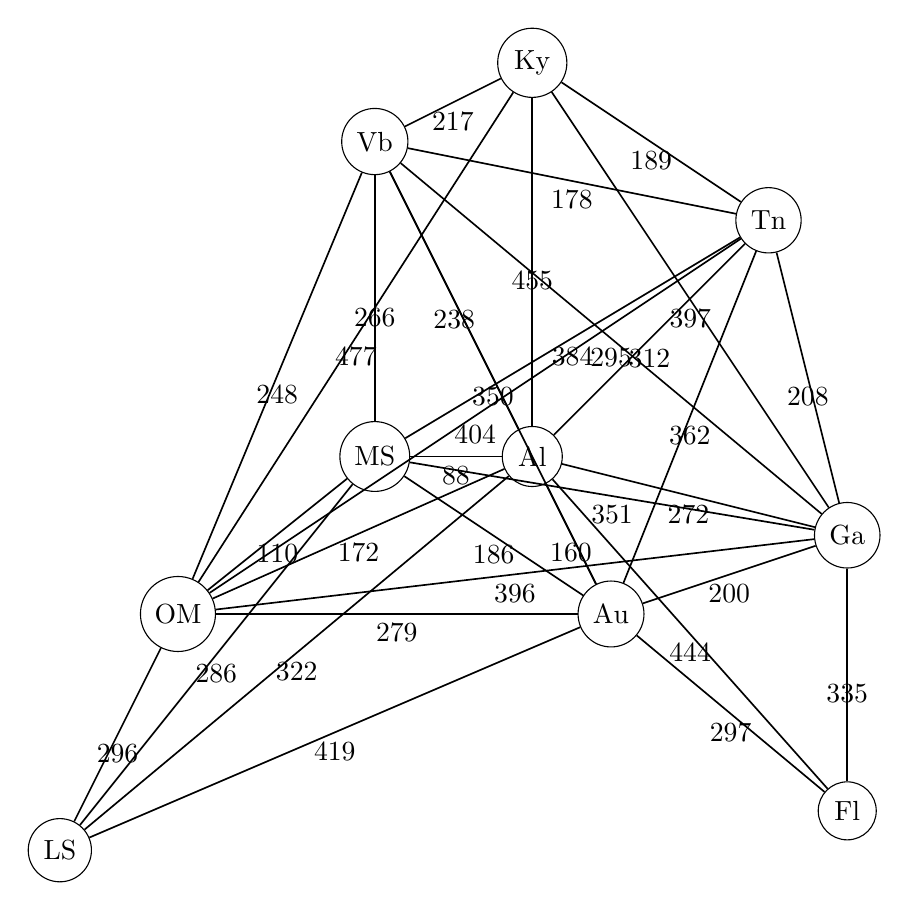
\begin{tikzpicture}
\begin{scope}[every node/.style = {circle, draw}]
\node (Al) at (6, 5) {Al};
\node (Au) at (7, 3) {Au};
\node (Fl) at (10, 0.5) {Fl};
\node (Ga) at (10, 4) {Ga};
\node (Ky) at (6, 10) {Ky};
\node (LS) at (0, 0) {LS};
\node (MS) at (4, 5) {MS};
\node (OM) at (1.5, 3) {OM};
\node (Tn) at (9, 8) {Tn};
\node (Vb) at (4, 9) {Vb};
\end{scope}
\begin{scope}[every edge/.style = {draw, semithick}]
\path (Al) edge node[anchor=north] {160} (Au);
\path (Al) edge node[anchor=north] {444} (Fl);
\path (Al) edge node[anchor=north] {272} (Ga);
\path (Al) edge node[anchor=north] {455} (Ky);
\path (Al) edge node[anchor=north] {322} (LS);
\path (Al) edge node[anchor=north] {88} (MS);
\path (Al) edge node[anchor=north] {172} (OM);
\path (Al) edge node[anchor=north] {312} (Tn);
\path (Al) edge node[anchor=north] {238} (Vb);
\path (Au) edge node[anchor=north] {297} (Fl);
\path (Au) edge node[anchor=north] {200} (Ga);
\path (Au) edge node[anchor=north] {419} (LS);
\path (Au) edge node[anchor=north] {186} (MS);
\path (Au) edge node[anchor=north] {279} (OM);
\path (Au) edge node[anchor=north] {362} (Tn);
\path (Au) edge node[anchor=north] {350} (Vb);
\path (Fl) edge node[anchor=north] {335} (Ga);
\path (Ga) edge node[anchor=north] {397} (Ky);
\path (Ga) edge node[anchor=north] {351} (MS);
\path (Ga) edge node[anchor=north] {396} (OM);
\path (Ga) edge node[anchor=north] {208} (Tn);
\path (Ga) edge node[anchor=north] {295} (Vb);
\path (Ky) edge node[anchor=north] {477} (OM);
\path (Ky) edge node[anchor=north] {189} (Tn);
\path (Ky) edge node[anchor=north] {217} (Vb);
\path (LS) edge node[anchor=north] {286} (MS);
\path (LS) edge node[anchor=north] {296} (OM);
\path (MS) edge node[anchor=north] {110} (OM);
\path (MS) edge node[anchor=north] {384} (Tn);
\path (MS) edge node[anchor=north] {266} (Vb);
\path (OM) edge node[anchor=north] {404} (Tn);
\path (OM) edge node[anchor=north] {248} (Vb);
\path (Tn) edge node[anchor=north] {178} (Vb);
\end{scope}
\end{tikzpicture}
\end{minipage}
}\vspace{5pt}\\

Solving following $\LP$ 
\begin{mini*}{x}{\sum_{e\in E_G}x_e}{}{}
    \addConstraint{\sum_{\{i,j\} \in \delta(i)} x_{\{i,j\}}}{=2, \quad}{\forall i \in V}
    \addConstraint{x}{\leq 1}
    \addConstraint{x}{\geq 0,}
\end{mini*}
i.e. using only degree constraints, we get:
\vspace{5pt}\\\scalebox{0.6}{
\begin{minipage}{\textwidth}
\centering
\begin{tikzpicture}
\begin{scope}[every node/.style = {circle, draw}]
\node (Al) at (6, 5) {Al};
\node (Au) at (7, 3) {Au};
\node (Fl) at (10, 0.5) {Fl};
\node (Ga) at (10, 4) {Ga};
\node (Ky) at (6, 10) {Ky};
\node (LS) at (0, 0) {LS};
\node (MS) at (4, 5) {MS};
\node (OM) at (1.5, 3) {OM};
\node (Tn) at (9, 8) {Tn};
\node (Vb) at (4, 9) {Vb};
\end{scope}
\begin{scope}[every edge/.style = {draw, semithick}]
\path (Al) edge node[anchor=north] {1.0} (LS);
\path (Al) edge node[anchor=north] {1.0} (MS);
\path (Au) edge node[anchor=north] {1.0} (Fl);
\path (Au) edge node[anchor=north] {1.0} (Ga);
\path (Fl) edge node[anchor=north] {1.0} (Ga);
\path (Ky) edge node[anchor=north] {1.0} (Tn);
\path (Ky) edge node[anchor=north] {1.0} (Vb);
\path (LS) edge node[anchor=north] {1.0} (OM);
\path (MS) edge node[anchor=north] {1.0} (OM);
\path (Tn) edge node[anchor=north] {1.0} (Vb);
\end{scope}
\end{tikzpicture}
\end{minipage}
}\vspace{5pt}\\

We see three subtours which we will eliminate by adding corresponding subtour constraints
\begin{align*}
\sum_{e \in \delta(S)} x_e &\geq 2, & \forall S &\in \{
\{\text{LS},\text{OM},\text{MS},\text{Al}\},
\{\text{Vb},\text{Ky},\text{Tn}\},
\{\text{Au},\text{Ga},\text{Fl}\},
\}\end{align*}

and get an integral Hamiltonian tour:
\vspace{5pt}\\\scalebox{0.6}{
\begin{minipage}{\textwidth}
\centering
\begin{tikzpicture}
\begin{scope}[every node/.style = {circle, draw}]
\node (Al) at (6, 5) {Al};
\node (Au) at (7, 3) {Au};
\node (Fl) at (10, 0.5) {Fl};
\node (Ga) at (10, 4) {Ga};
\node (Ky) at (6, 10) {Ky};
\node (LS) at (0, 0) {LS};
\node (MS) at (4, 5) {MS};
\node (OM) at (1.5, 3) {OM};
\node (Tn) at (9, 8) {Tn};
\node (Vb) at (4, 9) {Vb};
\end{scope}
\begin{scope}[every edge/.style = {draw, semithick}]
\path (Al) edge node[anchor=north] {1.0} (Au);
\path (Al) edge node[anchor=north] {1.0} (MS);
\path (Au) edge node[anchor=north] {1.0} (Fl);
\path (Fl) edge node[anchor=north] {1.0} (Ga);
\path (Ga) edge node[anchor=north] {1.0} (Tn);
\path (Ky) edge node[anchor=north] {1.0} (Tn);
\path (Ky) edge node[anchor=north] {1.0} (Vb);
\path (LS) edge node[anchor=north] {1.0} (MS);
\path (LS) edge node[anchor=north] {1.0} (OM);
\path (OM) edge node[anchor=north] {1.0} (Vb);
\end{scope}
\end{tikzpicture}
\end{minipage}
}\vspace{5pt}\\

Adding back all edges $V$ and modifying the constraints to include the new edges does indeed not 
generate a better solution:
\vspace{5pt}\\\scalebox{0.6}{
\begin{minipage}{\textwidth}
\centering
\begin{tikzpicture}
\begin{scope}[every node/.style = {circle, draw}]
\node (Al) at (6, 5) {Al};
\node (Au) at (7, 3) {Au};
\node (Fl) at (10, 0.5) {Fl};
\node (Ga) at (10, 4) {Ga};
\node (Ky) at (6, 10) {Ky};
\node (LS) at (0, 0) {LS};
\node (MS) at (4, 5) {MS};
\node (OM) at (1.5, 3) {OM};
\node (Tn) at (9, 8) {Tn};
\node (Vb) at (4, 9) {Vb};
\end{scope}
\begin{scope}[every edge/.style = {draw, semithick}]
\path (Al) edge node[anchor=north] {1.0} (Au);
\path (Al) edge node[anchor=north] {1.0} (MS);
\path (Au) edge node[anchor=north] {1.0} (Fl);
\path (Fl) edge node[anchor=north] {1.0} (Ga);
\path (Ga) edge node[anchor=north] {1.0} (Tn);
\path (Ky) edge node[anchor=north] {1.0} (Tn);
\path (Ky) edge node[anchor=north] {1.0} (Vb);
\path (LS) edge node[anchor=north] {1.0} (MS);
\path (LS) edge node[anchor=north] {1.0} (OM);
\path (OM) edge node[anchor=north] {1.0} (Vb);
\end{scope}
\end{tikzpicture}
\end{minipage}
}\vspace{5pt}\\

The total length of the optimal integral Hamilton tour is thus $2324$.
\subsection{Second instance}
First, have a look at our \enquote{good} graph $(V,E_G)$:
\vspace{5pt}\\\scalebox{0.6}{
\begin{minipage}{\textwidth}
\centering
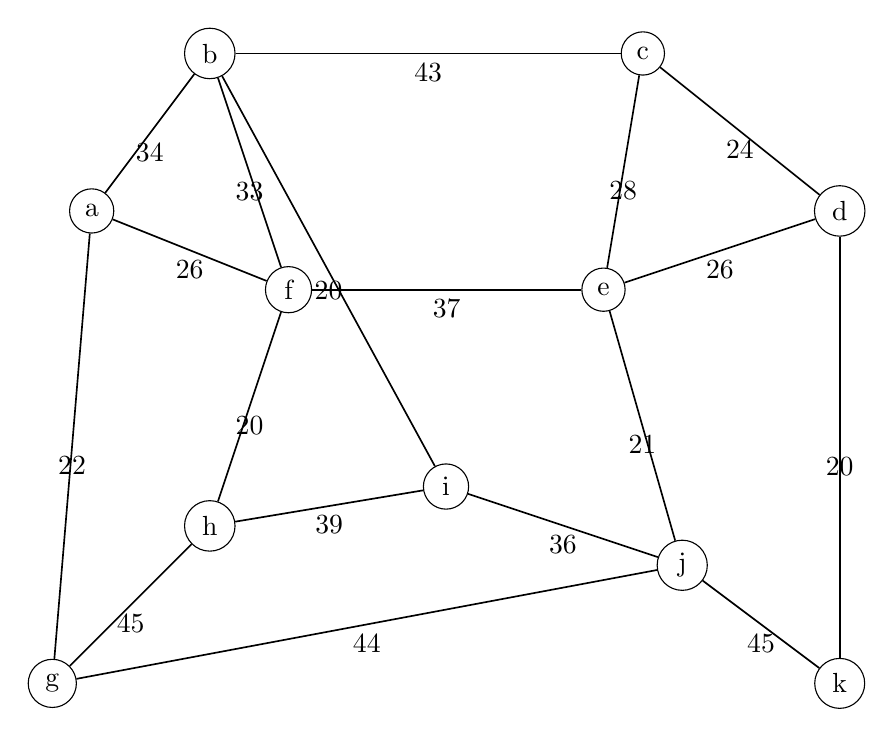
\begin{tikzpicture}
\begin{scope}[every node/.style = {circle, draw}]
\node (a) at (0.5, 6) {a};
\node (b) at (2, 8) {b};
\node (c) at (7.5, 8) {c};
\node (d) at (10, 6) {d};
\node (e) at (7, 5) {e};
\node (f) at (3, 5) {f};
\node (g) at (0, 0) {g};
\node (h) at (2, 2) {h};
\node (i) at (5, 2.5) {i};
\node (j) at (8, 1.5) {j};
\node (k) at (10, 0) {k};
\end{scope}
\begin{scope}[every edge/.style = {draw, semithick}]
\path (a) edge node[anchor=north] {34} (b);
\path (a) edge node[anchor=north] {26} (f);
\path (a) edge node[anchor=north] {22} (g);
\path (b) edge node[anchor=north] {43} (c);
\path (b) edge node[anchor=north] {33} (f);
\path (b) edge node[anchor=north] {20} (i);
\path (c) edge node[anchor=north] {24} (d);
\path (c) edge node[anchor=north] {28} (e);
\path (d) edge node[anchor=north] {26} (e);
\path (d) edge node[anchor=north] {20} (k);
\path (e) edge node[anchor=north] {37} (f);
\path (e) edge node[anchor=north] {21} (j);
\path (f) edge node[anchor=north] {20} (h);
\path (g) edge node[anchor=north] {45} (h);
\path (g) edge node[anchor=north] {44} (j);
\path (h) edge node[anchor=north] {39} (i);
\path (i) edge node[anchor=north] {36} (j);
\path (j) edge node[anchor=north] {45} (k);
\end{scope}
\end{tikzpicture}
\end{minipage}
}\vspace{5pt}\\

Solving following $\LP$ 
\begin{mini*}{x}{\sum_{e\in E_G}x_e}{}{}
    \addConstraint{\sum_{\{i,j\} \in \delta(i)} x_{\{i,j\}}}{=2, \quad}{\forall i \in V}
    \addConstraint{x}{\leq 1}
    \addConstraint{x}{\geq 0,}
\end{mini*}
i.e. using only degree constraints, we get:
\vspace{5pt}\\\scalebox{0.6}{
\begin{minipage}{\textwidth}
\centering
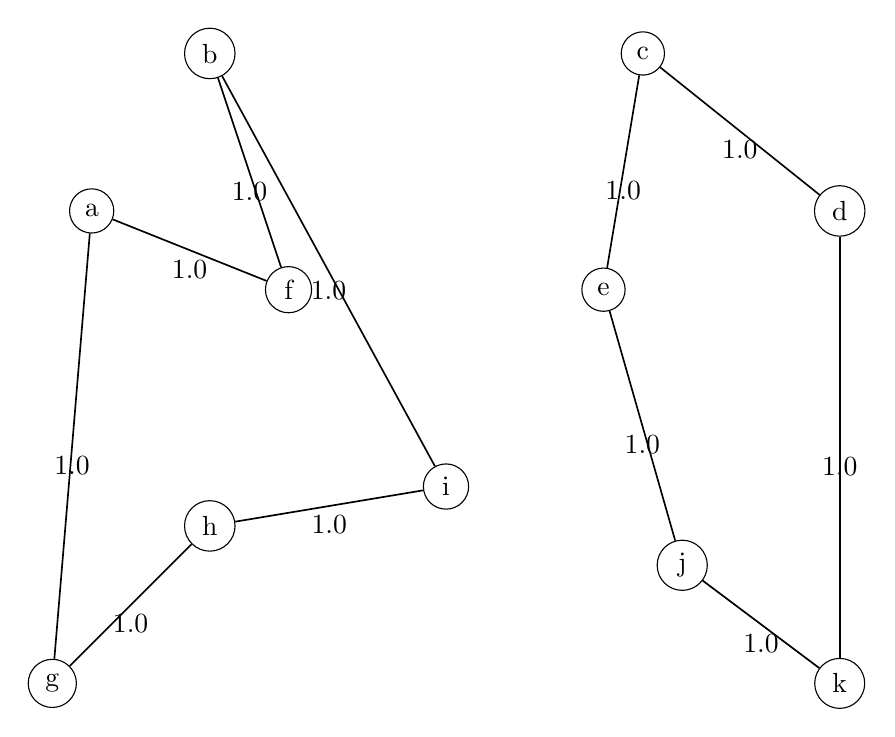
\begin{tikzpicture}
\begin{scope}[every node/.style = {circle, draw}]
\node (a) at (0.5, 6) {a};
\node (b) at (2, 8) {b};
\node (c) at (7.5, 8) {c};
\node (d) at (10, 6) {d};
\node (e) at (7, 5) {e};
\node (f) at (3, 5) {f};
\node (g) at (0, 0) {g};
\node (h) at (2, 2) {h};
\node (i) at (5, 2.5) {i};
\node (j) at (8, 1.5) {j};
\node (k) at (10, 0) {k};
\end{scope}
\begin{scope}[every edge/.style = {draw, semithick}]
\path (a) edge node[anchor=north] {1.0} (f);
\path (a) edge node[anchor=north] {1.0} (g);
\path (b) edge node[anchor=north] {1.0} (f);
\path (b) edge node[anchor=north] {1.0} (i);
\path (c) edge node[anchor=north] {1.0} (d);
\path (c) edge node[anchor=north] {1.0} (e);
\path (d) edge node[anchor=north] {1.0} (k);
\path (e) edge node[anchor=north] {1.0} (j);
\path (g) edge node[anchor=north] {1.0} (h);
\path (h) edge node[anchor=north] {1.0} (i);
\path (j) edge node[anchor=north] {1.0} (k);
\end{scope}
\end{tikzpicture}
\end{minipage}
}\vspace{5pt}\\

We see two subtours which we will eliminate by adding corresponding subtour constraints
\begin{align*}
\sum_{e \in \delta(S)} x_e &\geq 2, & \forall S &\in \{
\{\text{b},\text{a},\text{f},\text{i},\text{h},\text{g}\},
\{\text{c},\text{d},\text{e},\text{j},\text{k}\},
\}\end{align*}

and get following integral Hamiltonian path:
\vspace{5pt}\\\scalebox{0.6}{
\begin{minipage}{\textwidth}
\centering
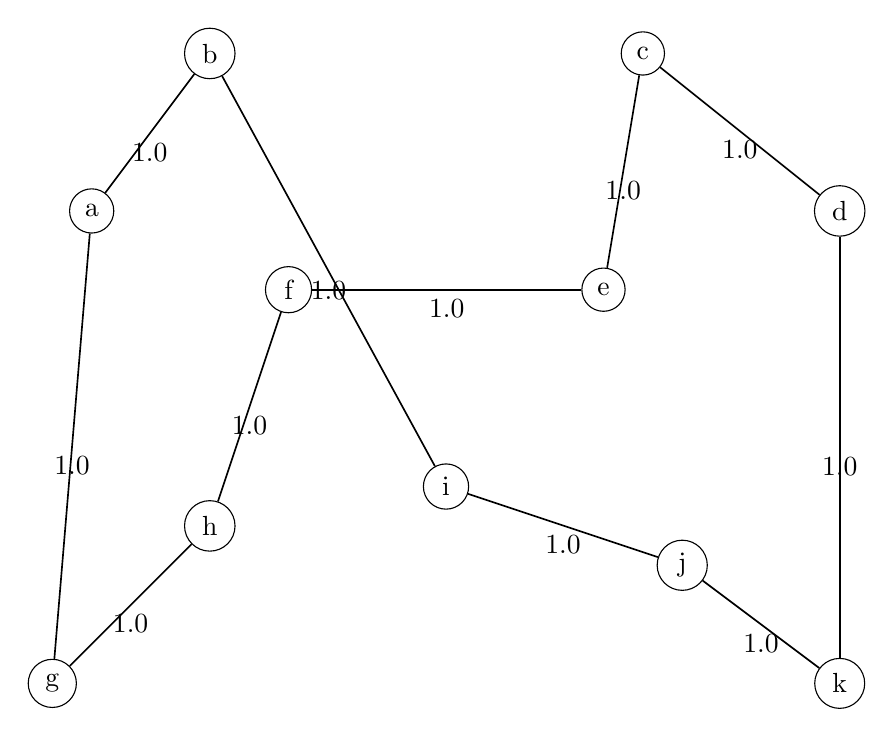
\begin{tikzpicture}
\begin{scope}[every node/.style = {circle, draw}]
\node (a) at (0.5, 6) {a};
\node (b) at (2, 8) {b};
\node (c) at (7.5, 8) {c};
\node (d) at (10, 6) {d};
\node (e) at (7, 5) {e};
\node (f) at (3, 5) {f};
\node (g) at (0, 0) {g};
\node (h) at (2, 2) {h};
\node (i) at (5, 2.5) {i};
\node (j) at (8, 1.5) {j};
\node (k) at (10, 0) {k};
\end{scope}
\begin{scope}[every edge/.style = {draw, semithick}]
\path (a) edge node[anchor=north] {1.0} (b);
\path (a) edge node[anchor=north] {1.0} (g);
\path (b) edge node[anchor=north] {1.0} (i);
\path (c) edge node[anchor=north] {1.0} (d);
\path (c) edge node[anchor=north] {1.0} (e);
\path (d) edge node[anchor=north] {1.0} (k);
\path (e) edge node[anchor=north] {1.0} (f);
\path (f) edge node[anchor=north] {1.0} (h);
\path (g) edge node[anchor=north] {1.0} (h);
\path (i) edge node[anchor=north] {1.0} (j);
\path (j) edge node[anchor=north] {1.0} (k);
\end{scope}
\end{tikzpicture}
\end{minipage}
}\vspace{5pt}\\

However, if we add all edges now, we get a non-integral solution
\vspace{5pt}\\\scalebox{0.6}{
\begin{minipage}{\textwidth}
\centering
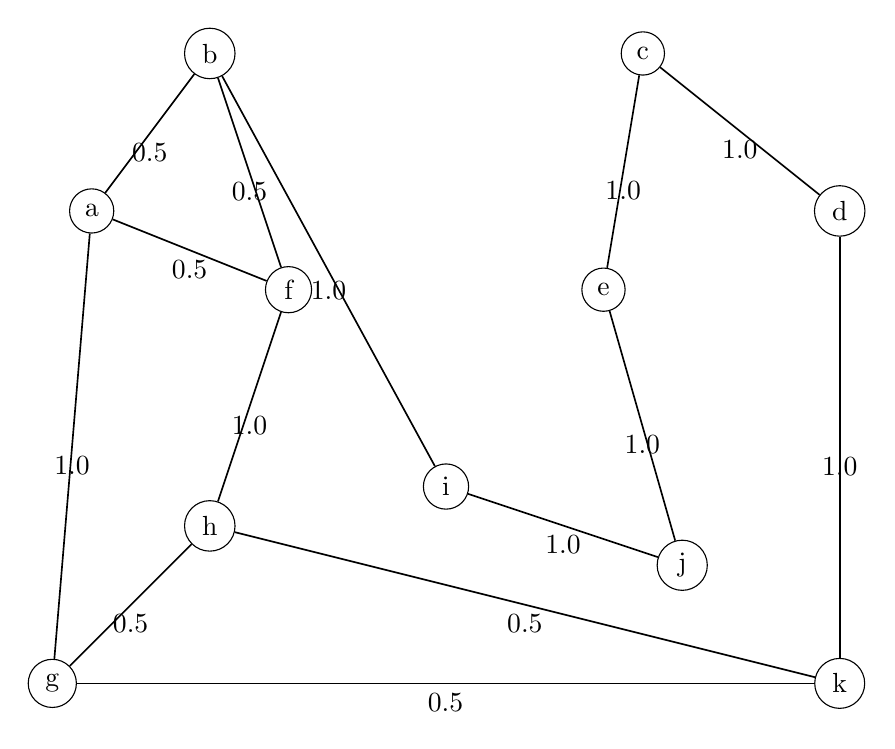
\begin{tikzpicture}
\begin{scope}[every node/.style = {circle, draw}]
\node (a) at (0.5, 6) {a};
\node (b) at (2, 8) {b};
\node (c) at (7.5, 8) {c};
\node (d) at (10, 6) {d};
\node (e) at (7, 5) {e};
\node (f) at (3, 5) {f};
\node (g) at (0, 0) {g};
\node (h) at (2, 2) {h};
\node (i) at (5, 2.5) {i};
\node (j) at (8, 1.5) {j};
\node (k) at (10, 0) {k};
\end{scope}
\begin{scope}[every edge/.style = {draw, semithick}]
\path (a) edge node[anchor=north] {0.5} (b);
\path (a) edge node[anchor=north] {0.5} (f);
\path (a) edge node[anchor=north] {1.0} (g);
\path (b) edge node[anchor=north] {0.5} (f);
\path (b) edge node[anchor=north] {1.0} (i);
\path (c) edge node[anchor=north] {1.0} (d);
\path (c) edge node[anchor=north] {1.0} (e);
\path (d) edge node[anchor=north] {1.0} (k);
\path (e) edge node[anchor=north] {1.0} (j);
\path (f) edge node[anchor=north] {1.0} (h);
\path (g) edge node[anchor=north] {0.5} (h);
\path (g) edge node[anchor=north] {0.5} (k);
\path (h) edge node[anchor=north] {0.5} (k);
\path (i) edge node[anchor=north] {1.0} (j);
\end{scope}
\end{tikzpicture}
\end{minipage}
}\vspace{5pt}\\

Therefore we add 2-matching constraints
\begin{align*}
x(E(H)) + x(D) &\leq 4, & H= \{\text{b},\text{a},\text{f}\},\ & D=\{\{\text{a},\text{g}\},\{\text{b},\text{i}\},\{\text{f},\text{h}\}\}\\
x(E(H)) + x(D) &\leq 4, & H= \{\text{h},\text{g},\text{k}\},\ & D=\{\{\text{a},\text{g}\},\{\text{f},\text{h}\},\{\text{d},\text{k}\}\}\\
\end{align*}

and still get a non-integral solution 
\vspace{5pt}\\\scalebox{0.6}{
\begin{minipage}{\textwidth}
\centering
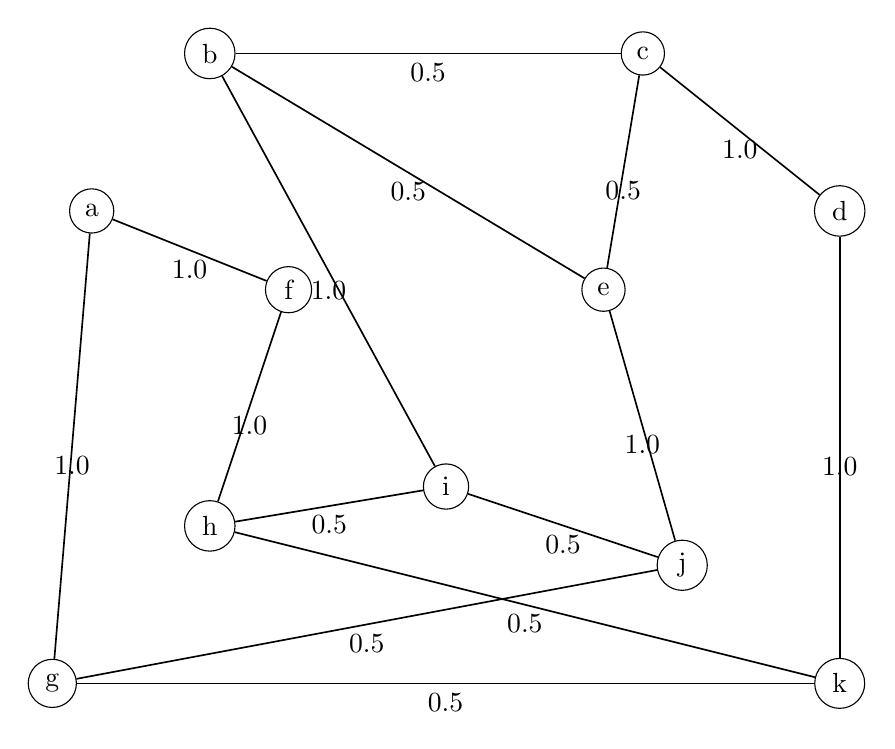
\begin{tikzpicture}
\begin{scope}[every node/.style = {circle, draw}]
\node (a) at (0.5, 6) {a};
\node (b) at (2, 8) {b};
\node (c) at (7.5, 8) {c};
\node (d) at (10, 6) {d};
\node (e) at (7, 5) {e};
\node (f) at (3, 5) {f};
\node (g) at (0, 0) {g};
\node (h) at (2, 2) {h};
\node (i) at (5, 2.5) {i};
\node (j) at (8, 1.5) {j};
\node (k) at (10, 0) {k};
\end{scope}
\begin{scope}[every edge/.style = {draw, semithick}]
\path (a) edge node[anchor=north] {1.0} (f);
\path (a) edge node[anchor=north] {1.0} (g);
\path (b) edge node[anchor=north] {0.5} (c);
\path (b) edge node[anchor=north] {0.5} (e);
\path (b) edge node[anchor=north] {1.0} (i);
\path (c) edge node[anchor=north] {1.0} (d);
\path (c) edge node[anchor=north] {0.5} (e);
\path (d) edge node[anchor=north] {1.0} (k);
\path (e) edge node[anchor=north] {1.0} (j);
\path (f) edge node[anchor=north] {1.0} (h);
\path (g) edge node[anchor=north] {0.5} (j);
\path (g) edge node[anchor=north] {0.5} (k);
\path (h) edge node[anchor=north] {0.5} (i);
\path (h) edge node[anchor=north] {0.5} (k);
\path (i) edge node[anchor=north] {0.5} (j);
\end{scope}
\end{tikzpicture}
\end{minipage}
}\vspace{5pt}\\

We add even more 2-matching constraints
\begin{align*}
x(E(H)) + x(D) &\leq 4, & H= \{\text{b},\text{c},\text{e}\},\ & D=\{\{\text{b},\text{i}\},\{\text{e},\text{j}\},\{\text{c},\text{d}\}\}\\
x(E(H)) + x(D) &\leq 7, & H= \{\text{h},\text{g},\text{k},\text{i},\text{j}\},\ & D=\{\{\text{a},\text{g}\},\{\text{f},\text{h}\},\{\text{d},\text{k}\},\{\text{b},\text{i}\},\{\text{e},\text{j}\}\}\\
\end{align*}

and finally get 
\vspace{5pt}\\\scalebox{0.6}{
\begin{minipage}{\textwidth}
\centering
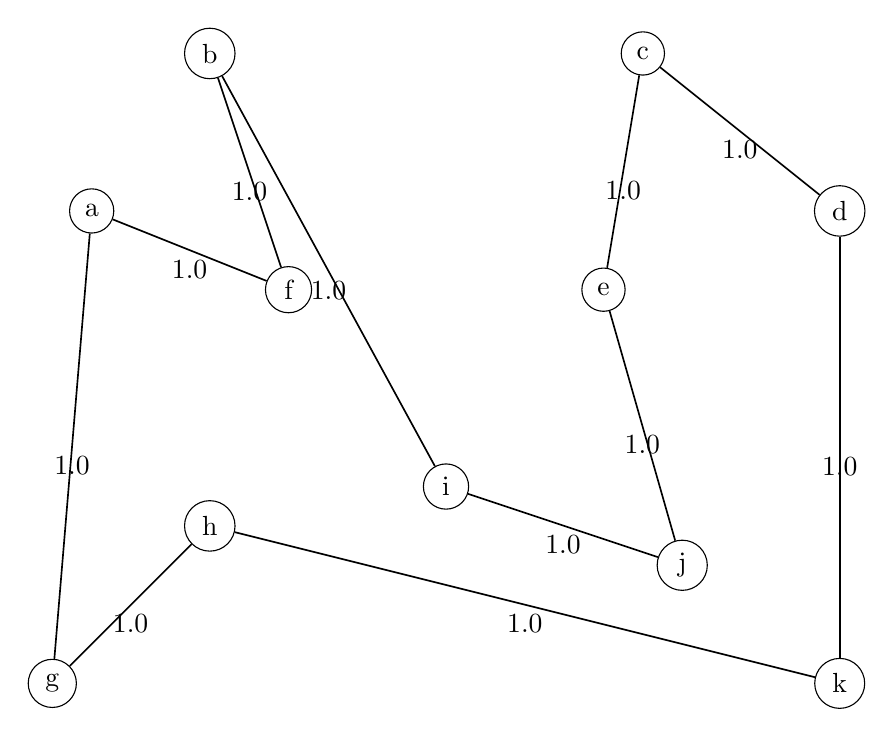
\begin{tikzpicture}
\begin{scope}[every node/.style = {circle, draw}]
\node (a) at (0.5, 6) {a};
\node (b) at (2, 8) {b};
\node (c) at (7.5, 8) {c};
\node (d) at (10, 6) {d};
\node (e) at (7, 5) {e};
\node (f) at (3, 5) {f};
\node (g) at (0, 0) {g};
\node (h) at (2, 2) {h};
\node (i) at (5, 2.5) {i};
\node (j) at (8, 1.5) {j};
\node (k) at (10, 0) {k};
\end{scope}
\begin{scope}[every edge/.style = {draw, semithick}]
\path (a) edge node[anchor=north] {1.0} (f);
\path (a) edge node[anchor=north] {1.0} (g);
\path (b) edge node[anchor=north] {1.0} (f);
\path (b) edge node[anchor=north] {1.0} (i);
\path (c) edge node[anchor=north] {1.0} (d);
\path (c) edge node[anchor=north] {1.0} (e);
\path (d) edge node[anchor=north] {1.0} (k);
\path (e) edge node[anchor=north] {1.0} (j);
\path (g) edge node[anchor=north] {1.0} (h);
\path (h) edge node[anchor=north] {1.0} (k);
\path (i) edge node[anchor=north] {1.0} (j);
\end{scope}
\end{tikzpicture}
\end{minipage}
}\vspace{5pt}\\

The total length is $319$.

\subsection{Code}
See the folder \texttt{exercises/code} in our project.
\label{sec:code_project}